\section{Gli algoritmi \textit{Nearest Neighbor}}

\subsection{\textit{Nearest Neighbor} (NN)}

\subsubsection{Definizione}
Verrà introdotto ora l'algoritmo di \textbf{\textit{Nearest Neighbor} (NN)} per la
classificazione binaria con \textit{feature} numeriche:
$$ \X = \RN^d \qquad\qquad \Y = \{-1,1\} $$

NN non è un'istanza di ERM in quanto non punta a minimizzare $\loss_S$.

\textbf{L'idea di NN è la sueguente:
\begin{itemize}
    \item Predici ogni punto del \textit{training set} con la propria etichetta;
    \item Predici gli altri punti con l'etichetta del punto del \textit{training set}
        che è più vicino al punto interessato.
\end{itemize}
}

Più formalmente, dato un \textit{training set}:
$$ S = \{(x_1,y_1),\dots,(x_m,y_m)\} $$
l'algoritmo $\Ann$ genera un classificatore $\hnn:\RN \rightarrow \{-1,1\}$ definito
come segue:
$$ \hnn(x) = \text{etichetta $y_t$ del punto $x_t \in S$ più vicino a x} $$

Se a minimizzare la distanza con $x$ sono più punti, si predirrà l'etichetta più
presente tra i putni vicini. Se non c'è una maggioranza di etichette tra i punti
più vicini si predirrà un valore di default $\in \{-1,1\}$.

Presi due punti $x=(x_1,\dots,x_d)$ e $x_t=(x_{t,1},\dots,x_{t,d})$, la distanza
$||x-x_t||$ verrà calcolata tramite la distanza euclidea:
$$||x-x_t|| = \sqrt{\sum_{i=1}^d (x_i-x_{t,i})^2}$$

Ogni classificatore binario $\pred : \RN^d \rightarrow \{-1,1\}$ partiziona $\RN^d$
in due regioni (come mostrato in figura \ref{fig:voronoi}):
$$ \colorbox{transp-cyan}{$\{ x \in \RN^d : \pred(x)=1 \}$} \quad , \quad 
   \colorbox{transp-orange}{$\{ x \in \RN^d : \pred(x)=-1 \}$} $$

\begin{figure}[h]
    \centering
    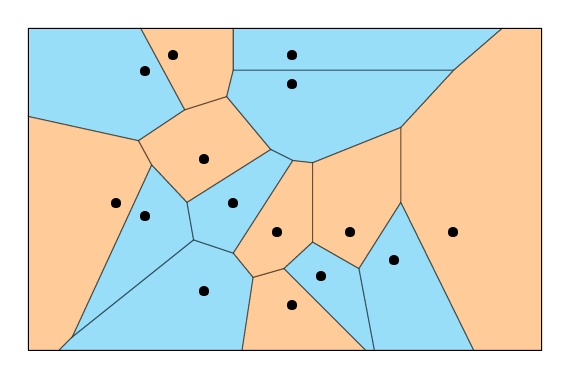
\begin{tikzpicture}[scale=2.8]

    \draw[fill=cyan,opacity=.4](-0.33, 1.33)--(0.18, 1.33)--(0.38, 0.96)--(0.17, 0.82)--(-0.33, 0.93)--(-0.33, 1.33);
    \draw[fill=orange,opacity=.4](-0.33, -0.13)--(-0.33, 0.93)--(0.17, 0.82)--(0.23, 0.71)--(-0.13, -0.07)--(-0.19, -0.13)--(-0.33, -0.13);
    \draw[fill=cyan,opacity=.4](-0.19, -0.13)--(-0.13, -0.07)--(0.42, 0.37)--(0.6, 0.31)--(0.69, 0.2)--(0.64, -0.13)--(-0.19, -0.13);
    \draw[fill=orange,opacity=.4](0.38, 0.96)--(0.57, 1.02)--(0.77, 0.78)--(0.39, 0.54)--(0.23, 0.71)--(0.17, 0.82)--(0.38, 0.96);
    \draw[fill=cyan,opacity=.4](0.23, 0.71)--(0.39, 0.54)--(0.42, 0.37)--(-0.13, -0.07)--(0.23, 0.71);
    \draw[fill=orange,opacity=.4](0.6, 1.33)--(0.6, 1.14)--(0.57, 1.02)--(0.38, 0.96)--(0.18, 1.33)--(0.6, 1.33);
    \draw[fill=cyan,opacity=.4](0.57, 1.02)--(0.6, 1.14)--(1.6, 1.14)--(1.36, 0.88)--(0.96, 0.72)--(0.87, 0.73)--(0.77, 0.78)--(0.57, 1.02);
    \draw[fill=orange,opacity=.4](0.64, -0.13)--(0.69, 0.2)--(0.83, 0.24)--(1.2, -0.13)--(0.64, -0.13);
    \draw[fill=cyan,opacity=.4](0.87, 0.73)--(0.6, 0.31)--(0.42, 0.37)--(0.39, 0.54)--(0.77, 0.78)--(0.87, 0.73);
    \draw[fill=orange,opacity=.4](0.6, 0.31)--(0.87, 0.73)--(0.96, 0.72)--(0.96, 0.36)--(0.83, 0.24)--(0.69, 0.2)--(0.6, 0.31);
    \draw[fill=cyan,opacity=.4](1.2, -0.13)--(0.83, 0.24)--(0.96, 0.36)--(1.17, 0.24)--(1.24, -0.13)--(1.2, -0.13);
    \draw[fill=cyan,opacity=.4](1.82, 1.33)--(1.6, 1.14)--(0.6, 1.14)--(0.6, 1.33)--(1.82, 1.33);
    \draw[fill=orange,opacity=.4](1.36, 0.88)--(1.36, 0.54)--(1.17, 0.24)--(0.96, 0.36)--(0.96, 0.72)--(1.36, 0.88);
    \draw[fill=orange,opacity=.4](2.0, 1.33)--(2.0, -0.13)--(1.69, -0.13)--(1.36, 0.54)--(1.36, 0.88)--(1.6, 1.14)--(1.82, 1.33)--(2.0, 1.33);
    \draw[fill=cyan,opacity=.4](1.24, -0.13)--(1.17, 0.24)--(1.36, 0.54)--(1.69, -0.13)--(1.24, -0.13);
    \draw (-0.33, -0.13)--(2.0, -0.13)--(2.0, 1.33)--(-0.33, 1.33)--(-0.33, -0.13);
    \node at (0.87, 1.2) {\textbullet};
    \node at (0.2, 1.13) {\textbullet};
    \node at (1.13, 0.4) {\textbullet};
    \node at (0.87, 0.07) {\textbullet};
    \node at (0.47, 0.73) {\textbullet};
    \node at (0.2, 0.47) {\textbullet};
    \node at (0.8, 0.4) {\textbullet};
    \node at (0.6, 0.53) {\textbullet};
    \node at (0.87, 1.07) {\textbullet};
    \node at (1.33, 0.27) {\textbullet};
    \node at (0.07, 0.53) {\textbullet};
    \node at (0.33, 1.2) {\textbullet};
    \node at (1.6, 0.4) {\textbullet};
    \node at (0.47, 0.13) {\textbullet};
    \node at (1.0, 0.2) {\textbullet};

\end{tikzpicture}
    \caption{Diagramma di Voronoi in $\RN^2$\label{fig:voronoi}; tutti i punti $x$
    interni a una cella con centro \textbullet $x_t$ sono tali che $\hnn(x)=y_t$}
\end{figure}

\subsubsection{Efficienza ed efficacia}

Siccome il funzionamento di NN implica la memorizzazione di tutto il 
\textit{training set}, \textbf{l'algoritmo non scala bene con il numero di
$|S| = m$ di \textit{training point}}. Inoltre, calcolare un qualsiasi
$\hnn(x)$ è costoso, in quanto richiede di calcolare la distanza tra $x$ e
tutti gli altri punti di $S$; questo in $\RN^d$ comporta un costo di 
$\Theta (dm)$.

Infine, si noti come, vista la completa memorizzazione di $S$, \textbf{NN generi 
sempre un classificatore $\hnn$ con \textit{training error} nullo}:
$$ \loss_S(\hnn)=0 $$

\subsection{\texorpdfstring{$k-$Nearest Neighbor (\kNN)}{k-NN}}

\subsubsection{Definizione}
Partendo dagli algoritmi NN, si può ottenere una famiglia di algoritmi detta
\kNN; il parametro $k$ assume tipicamente i valori $k=1,3,5,\dots$ con $k<|S|$.

Questi algoritmi sono definiti come segue: dato un \textit{training set} $S$ e un
punto $x \in \X$, \kNN \ genererà un predittore $\hknn$ tale che:
$$\hknn(x) = \text{etichetta $y_t$ appartenente alla maggioranza dei $k$ punti
più vicini a $x$} $$

\begin{figure}[h]
    \centering
    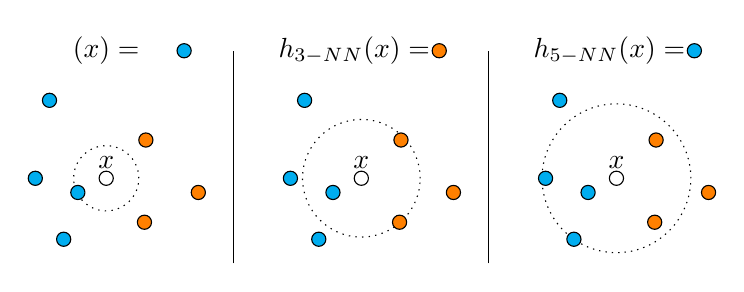
\begin{tikzpicture}[scale=1.8]

    \def \r {.05}

    \begin{scope}
        \coordinate (X) at (1.4,1.6);

        \node at (1.4,2.5) {$\hnn(x)=$};
        \draw[fill=cyan] (1.95,2.5) circle (\r);

        \draw[dash pattern=on .5pt off 1.89pt](X) circle (.23);

        \draw[fill=white] (X)  circle (\r) node[above]{$x$};
    
        \draw[fill=cyan]   (.9,1.6)    circle (\r);
        \draw[fill=cyan]   (1.0,2.15)  circle (\r);
        \draw[fill=cyan]   (1.1,1.17)  circle (\r);
        \draw[fill=cyan]   (1.2,1.5)   circle (\r);
        \draw[fill=orange] (1.68,1.87) circle (\r);
        \draw[fill=orange] (1.67,1.29) circle (\r);
        \draw[fill=orange] (2.05,1.5)  circle (\r);

        \draw (2.3,1) -- (2.3,2.5);
    \end{scope}

    \begin{scope}[xshift=1.8cm]
        \coordinate (X) at (1.4,1.6);

        \node at (1.35,2.5) {$h_{3\text{-NN}}(x)=$};
        \draw[fill=orange] (1.95,2.5) circle (\r);

        \draw[dash pattern=on .5pt off 1.89pt](X) circle (.415);

        \draw[fill=white] (X)  circle (\r) node[above]{$x$};
    
        \draw[fill=cyan]   (.9,1.6)    circle (\r);
        \draw[fill=cyan]   (1.0,2.15)  circle (\r);
        \draw[fill=cyan]   (1.1,1.17)  circle (\r);
        \draw[fill=cyan]   (1.2,1.5)   circle (\r);
        \draw[fill=orange] (1.68,1.87) circle (\r);
        \draw[fill=orange] (1.67,1.29) circle (\r);
        \draw[fill=orange] (2.05,1.5)  circle (\r);

        \draw (2.3,1) -- (2.3,2.5);
    \end{scope}

    \begin{scope}[xshift=3.6cm]
        \coordinate (X) at (1.4,1.6);
        
        \node at (1.35,2.5) {$h_{5\text{-NN}}(x)=$};
        \draw[fill=cyan] (1.95,2.5) circle (\r);

        \draw[dash pattern=on .5pt off 1.815pt](X) circle (.525);

        \draw[fill=white] (X)  circle (\r) node[above]{$x$};
    
        \draw[fill=cyan]   (.9,1.6)    circle (\r);
        \draw[fill=cyan]   (1.0,2.15)  circle (\r);
        \draw[fill=cyan]   (1.1,1.17)  circle (\r);
        \draw[fill=cyan]   (1.2,1.5)   circle (\r);
        \draw[fill=orange] (1.68,1.87) circle (\r);
        \draw[fill=orange] (1.67,1.29) circle (\r);
        \draw[fill=orange] (2.05,1.5)  circle (\r);
    \end{scope}

\end{tikzpicture}
    \caption{Esempi di $\hknn$ con $\X=\RN^2$; si noti come, con lo stesso 
    \textit{training set}, la predizione cambia al variare di $k$. \label{fig:knn}}
\end{figure}
\vspace{1em}

\subsubsection{Efficienza ed efficacia}

A livello di efficienza \kNN \ soffre degli stessi problemi di NN vista la
memorizzazione dell'intero \textit{training set}.

Per quanto riguarda la sua efficacia invece, \kNN \ non ha sempre un 
\textit{training error} nullo:
$$ \loss_S(\hknn)\geq0 $$

\begin{figure}[h]
    \centering
    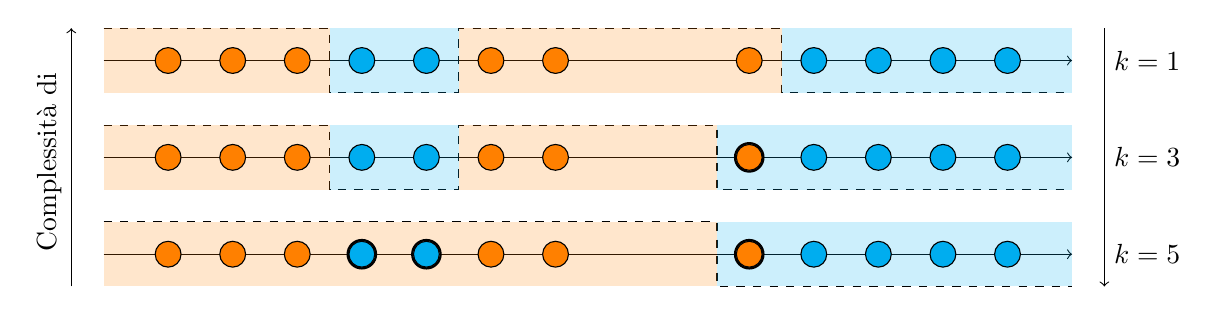
\begin{tikzpicture}[scale=.82]
    
    \def \r {.2}
    
    \draw[->] (0,3) -- (15,3);
    \draw[->] (0,1.5) -- (15,1.5);
    \draw[->] (0,0) -- (15,0);

    \draw[dashed] (0,3.5)--(3.5,3.5)--(3.5,2.5)--(5.5,2.5)--(5.5,3.5)
        --(10.5,3.5)--(10.5,2.5)--(15,2.5);
    \fill[orange, opacity=.2] (0,3.5)   rectangle (3.5,2.5);
    \fill[orange, opacity=.2] (5.5,3.5) rectangle (10.5,2.5);
    \fill[cyan  , opacity=.2] (3.5,3.5) rectangle (5.5,2.5);
    \fill[cyan  , opacity=.2] (10.5,3.5) rectangle (15,2.5);

    \draw[dashed] (0,2)--(3.5,2)--(3.5,1)--(5.5,1)--(5.5,2)
        --(9.5,2)--(9.5,1)--(15,1);
    \fill[orange, opacity=.2] (0   ,2) rectangle (3.5 ,1);
    \fill[orange, opacity=.2] (5.5 ,2) rectangle (9.5,1);
    \fill[cyan  , opacity=.2] (3.5 ,2) rectangle (5.5 ,1);
    \fill[cyan  , opacity=.2] (9.5,2) rectangle (15  ,1);

    \draw[dashed] (0,.5)--(9.5,.5)--(9.5,-.5)--(15,-.5);
    \fill[orange, opacity=.2] (0  ,.5) rectangle (9.5,-.5);
    \fill[cyan  , opacity=.2] (9.5,.5) rectangle (15 ,-.5);

    \draw[thick] (10,1.5) circle (\r+.02);
    \draw[thick] (4 ,0)   circle (\r+.02);
    \draw[thick] (5 ,0)   circle (\r+.02);
    \draw[thick] (10,0)   circle (\r+.02);

    \foreach \y in {3,1.5,0} {
        \draw[fill=orange] (1, \y) circle (\r);
        \draw[fill=orange] (2, \y) circle (\r);
        \draw[fill=orange] (3, \y) circle (\r);
        \draw[fill=cyan]   (4, \y) circle (\r);
        \draw[fill=cyan]   (5, \y) circle (\r);
        \draw[fill=orange] (6, \y) circle (\r);
        \draw[fill=orange] (7, \y) circle (\r);
        \draw[fill=orange] (10,\y) circle (\r);
        \draw[fill=cyan]   (11,\y) circle (\r);
        \draw[fill=cyan]   (12,\y) circle (\r);
        \draw[fill=cyan]   (13,\y) circle (\r);
        \draw[fill=cyan]   (14,\y) circle (\r);
    }
    
    \draw[->] (-.5,-.5) -- (-.5,3.5);
    \node[rotate=90,above] at (-.5,1.5) {Complessità di $\hknn$};
    \draw[->] (15.5,3.5) -- (15.5,-.5);
    \node[right] at (15.5,3)   {$k=1$};
    \node[right] at (15.5,1.5) {$k=3$};
    \node[right] at (15.5,0)   {$k=5$};

\end{tikzpicture}
    \caption{\label{fig:knn_line}Esempi di $\hknn$ con $\X = \RN$.}
\end{figure}
\vspace{1em}

Come si può infatti notare dalla figura \ref{fig:knn_line}, nei casi con $k=3$ e 
$k=5$ sono presenti punti errati (evidenziati in grassetto) considerati dal 
classificatore come \textit{outlier}. Inoltre \textbf{al crescere di $k$ cresce 
anche la \quotes{semplicità} del classificatore così come il numero di punti errati}.
L'estremo di ciò è quando $k=|S|$; in questo caso infatti $\hknn$ diventa un 
classificatore costante che predice sempre l'etichetta più presente in tutto $S$.

In un generico classificatore $\hknn$ tipicamente succede che:
\begin{itemize}
    \item \textbf{Se $k$ è troppo basso} si ottiene un classificatore che si 
        \quotes{fida} troppo del \textit{training set}, ottenendo quindi 
        \textbf{\textit{overfitting}};
    \item \textbf{Se $k$ è troppo alto}, si ottiene un classificatore troppo
        semplice, ottenendo \textbf{\textit{underfitting}}.
\end{itemize}

Tutti i classificatori introdotti fino ad'ora sono classificatori binari ($|\Y|=2$).
Tuttavia \kNN può essere usato anche per:
\begin{itemize}
    \item problemi di classificazione multiclasse ($|\Y|>2$): si opera come nel caso
        binario, predicendo quindi l'etichetta più presente nei $k$ punti più vicini;
    \item problemi di regressione ($\Y = \RN$): si predice la media aritmetice delle
        etichette dei $k$ punti più vicini.
\end{itemize}